\newpage
\section{Problema 1: Algoritmo Exacto para 2-List Coloring}

\subsection{Descripción de la problemática}
Este ejericicio está centrado en la resolución de un problema particular de coloreo, 2-listColoring. En este caso, cada nodo se puede colorear solo con uno o dos colores específicos. El algoritmo debe determinar si existe o no un coloreo en donde no existen dos nodos consecutivos del mismo color y, en caso afirmativo, encontrar una solución.
Este problema es facilmente reducible a 2-SAT, por lo cual existen algortmos polinomiales que lo resuelven.

\subsection{Resolución propuesta y justificación}
Como mencionamos antes, el problema del 2-ListColoring es fácilmente reducible a un problema de 2-SAT, y en esto se basa el algoritmo implementado. Si existe una coloración posible, entonces el hecho de que un determinado nodo esté pintado de un color implica que ninguno de sus vecinos esta pintado del mismo. Además, si un nodo tiene dos colores posibles, el nodo esta pintado de un color C1 si y solo si no esta pintado del color C2.
El 2-SAT se representa con un grafo dirigido en donde un nodo A (que representa una proposición) apunta a un nodo B si A implica B.

Sean x, y, z proposiciones representadas por nodos de nuestro grafo dirigido, si en el grafo existe una arista desde el nodo que representa a x al nodo que representa a y, y otra arista entre el nodo que representa a y al nodo que representa a z, esto significa que x $\rightarrow$ y e y $\rightarrow$ z, de lo cual se deduce que x $\rightarrow$ z. Generalizando se puede decir que, dadas x, z proposiciones,  x $\rightarrow$ z si y solo si existe un camino desde el nodo que representa a x hasta el nodo que representa a z. Es decir, en este contexto una componente fuertemente conexa representa un conjunto de proposiciones de las cuales se puede afirmar que todas son válidas o todas son falsas. 

Para la resolución del 2-SAT, se implementa el algoritmo de Kosaraju. Este algoritmo recibe como entrada un grafo dirigido y devuelve como resultado las componentes fuertemente conexas que se encuentran en el mismo. 

Como el algoritmo de Kosaraju encuentra todas las componentes fuertemente conexas, entonces, dadas dos componentes C1 y C2, si existe un camino entre C1 y C2, no puede existir un camino desde C2 a C1 (de lo contrario ambas debería estar en la misma componente). Además, si existe un camino entre C1 y C2, con el algoritmo de Kosaraju C1 será detectada antes que C2. Nuestra implementación fue diseñada para que la lista de componentes fuertemente conexas resultante del algoritmo preserve este orden de detección. Posteriormente de la ejecución del Kosaraju, nuestro algoritmo registra, para cada componente conexa, cual es la componente conexa que contiene la negación de sus proposiciones. En caso de que una misma componente conexa contenga a una proposición y su negación, entonces se determina que el problema no tiene solución, ya que implicaría que, sea x la proposición en cuestión, x $\leftrightarrow$ $\lnot$x.

Finalmente comienzan a fijarse los valores de verdad, recorriendo las componentes fuertemente conexas en el orden en que fueron obtenidas en el paso anterior. Si a la componente aún no se le asignó un valor de verdad, se le asigna false. Cuando se fija un valor para una componente determinada, a la componente que contiene la negación de sus proposiciones se le asigna el valor opuesto.  Además, si a una componente se le asigna false, todos las componentes que implican a la misma (es decir, todas las componentes desde las cuales existe un camino hasta la componente evaluada) también se les asigna false (recursivamente). Y, si a una componente se le asigna true, a todas las componentes que son implicadas por la misma se  les asigna también true. Si el algoritmo encuentra una contradicción (es decir, una componente que a la que se busca  asignar false ya tiene true o viceversa), determina que el problema no tiene solución.

Una vez determinados los valores de verdad, se deduce la coloración de los nodos del grafo original a partir de las proposiciones que forman parte de las componentes evaluadas como verdaderas.

\newcommand{\pushcode}[1][1]{\hskip\dimexpr#1\algorithmicindent\relax}
\subsection{PseudoCódigo}

A continuación se presenta el pseudocódigo para 2-List Coloring:

\noindent \textbf{Function} {algoritmo2ListColoring($grafoOriginal$)}
\begin{algorithmic}
	\STATE {$grafoDirigido$ = crearGrafoDirigidoConProposiciones($grafoOriginal$)}
	\STATE {$listaComponentesConexas$ =  Kosaraju($grafoDirigido$)}
	\STATE {$grafoCompacto$ = generarGrafoCompacto($listaComponentesConexas$)}
	\IF {$grafoCompacto$ es INVALIDO}
		\RETURN {NO_HAY_SOLUCION}
	\ENDIF
	\STATE {$asignacionDeVerdad$ = asignarValoresDeVerdad($listaComponentesConexas$, $grafoCompacto$)}
	\IF {$asignacionDeVerdad==$INVALIDO}
		\RETURN {NO_HAY_SOLUCION}
	\ENDIF
	\RETURN {obtenerColoreoParaGrafoOriginal($listaComponentesConexas$)}
\end{algorithmic}
\textbf{EndFunction}

\vspace{5mm}

\noindent \textbf{Function} {crearGrafoDirigidoConProposiciones($grafoOriginal$)}
\begin{algorithmic}
	\STATE {$grafoDirigido$ = VACIO}
	\FOR {cada nodo $A$ del $grafoOriginal$}
		\IF {cantidadColores($A$)$==$1}
			\STATE {$grafoDirigido$.agregar($\lnot A$color $\rightarrow$ $A$color)}
		\ELSE
			\STATE {$grafoDirigido$.agregar($A$color1 $\leftrightarrow$ $\lnot A$color2)}
			\STATE {$grafoDirigido$.agregar($A$color2 $\leftrightarrow$ $\lnot A$color1)}
		\ENDIF
	\ENDFOR
	\FOR {cada arista $(A,B)$}
		\FOR {cada color comun $c$ entre $A$ y $B$}
			\STATE {$grafoDirigido$.agregar($Ac$ $\rightarrow$ $\lnot Bc$)}
			\STATE {$grafoDirigido$.agregar($Bc$ $\rightarrow$ $\lnot Ac$)}
		\ENDFOR
	\ENDFOR
	\RETURN {$grafoDirigido$}
\end{algorithmic}
\textbf{EndFunction}

\vspace{5mm}

\noindent \textbf{Function} {Kosaraju($grafoDirigido$)}
\begin{algorithmic}
	\STATE {$listaComponentesConexas$ = VACIO}
	\STATE {$pila$ = VACIO}
	\FOR {cada nodo $A$ de $grafoDirigido$}
		\IF {($pila$ no contiene $A$)}
			\STATE {apilar nodos partiendo de $A$ utilizando BFS}
		\ENDIF
	\ENDFOR

	\STATE {$grafoDirigidoInverso$ = $grafoDirigido$.invertirAristas()}

	\WHILE {$pila$ no vacia}
		\STATE {$A$ = $pila$.SacarPrimero}
		\IF {(no marcada $A$)}
			\STATE {$componente$ = VACIO}
			\STATE {agregar a $componente$ todos los nodos partiendo de $A$ utilizando BFS en $grafoDirigidoInverso$}
			\STATE {marcar($A$)}
			\STATE {$listaComponentesConexas$.agrefarAlFinal($componente$)}
		\ENDIF
	\ENDWHILE

	\RETURN {$listaComponentesConexas$}
\end{algorithmic}
\textbf{EndFunction}

\vspace{5mm}

\noindent \textbf{Function} {generarGrafoCompacto($listaComponentesConexas$)}
\begin{algorithmic}
	\STATE {$grafoCompacto$ = VACIO}
	\FOR {cada $componente$ en $listaComponentesConexas$}
		\FOR {cada nodo $A$ de $componente$}
			\FOR {cada arista $(A,B)$}
				\STATE {$componente$.agregarArista(componenteDe($B$))}
			\ENDFOR
			\FOR {cada nodo $B$ negado por $A$}
				\STATE {$componente$.asociarComoNegacion(componenteDe($B$))}
				\STATE {componenteDe($B$).asociarComoNegacion($componente$)}

				\IF {$componente$==componenteDe(B)}
					\RETURN {INVALIDO}
				\ENDIF
			\ENDFOR
		\ENDFOR
	\ENDFOR
	\RETURN {$grafoCompacto$}
\end{algorithmic}
\textbf{EndFunction}

\vspace{5mm}

\noindent \textbf{Function} {asignarValoresDeVerdad($listaComponentesConexas$, $grafoCompacto$)}
\begin{algorithmic}
	\FOR {cada $componente$ en $listaComponentesConexas$}
		\IF {no esta marcada $componente$}
			\STATE {marcar($componente$, FALSE)}
			\STATE {propagar FALSE a todas las componentes que poseen un camino hasta \\
			\pushcode[2] esta $componente$ en $grafoCompacto$}
			\IF {inconsistencia al propagar}
				\RETURN {INVALIDO}
			\ENDIF
			\STATE {marcar($componente$.negacionAsociada, TRUE)}
			\STATE {propagar TRUE a todas las componentes accesibles desde \\
			\pushcode[2] $componente$.negacionAsociada en $grafoCompacto$}
			\IF {inconsistencia al propagar}
				\RETURN {INVALIDO}
			\ENDIF
		\ENDIF
	\ENDFOR
	\RETURN {VALIDO}
\end{algorithmic}
\textbf{EndFunction} 

\vspace{5mm}

\noindent \textbf{Function} {obtenerColoreoParaGrafoOriginal($listaComponentesConexas$)}
\begin{algorithmic}
	\STATE {$colores$ = VACIO}
	\FOR {cada $componente$ con valor TRUE en $listaComponentesConexas$}
		\FOR {cada $nodo$ con proposicion afirmativa de $componente$}
			\STATE {$colores$.asignarColor($nodo$.nodoDeGrafoOriginal.identidad, $nodo$.proposicion.colorPropuesto)}
		\ENDFOR
	\ENDFOR
	\RETURN {$colores$}
\end{algorithmic}
\textbf{EndFunction}

\subsection{Análisis de la complejidad}
El grafo dirigido contiene a los sumo cuatro veces más nodos que el grafo de entrada, y el grafo compacto tiene a los sumo tantos nodos como el grafo dirigido. Por lo tanto, podemos afirmar que, sea n la cantidad de nodos inicial, n' la cantidad de nodos del grafo dirigido y n'' la cantidad de nodos del grafo compacto, $\mathcal{O}(f(n)) = \mathcal{O}(f(n')) = \mathcal{O}(f(n''))$ (si no se conocen datos adicionales para la entrada).

Generar el grafo dirigido a partir del grafo de entrada tiene una complejidad de $\mathcal{O}(n^2\log{n})$, ya que para cada nodo del grafo, es necesario crear los nodos dirigidos que lo representan y definir sus aristas con otros nodos. A medida que se van creando, los nodos se guardan y se buscan en un TreeSet.

El algoritmo utilizado para encontrar las componentes fuertemente conexas no recorre más de dos veces todos los nodos, por lo cual su complejidad es lineal, al igual que el algoritmo que determina el valor de verdad de los nodos compactos.

\subsection{Experimentación}
Casos de test:
\subsubsection{El triángulo}
En este test existen tres nodos interconextados en donde cada nodo comparte un color con uno de sus vecinos. El algoritmo debería encontrar la única solución posible.
Posteriormente, se le añade al triangulo un nodo extra vecino del primero con el color con el cual estaba pintado el primero, con lo cual no existe solución.
\subsubsection{El pentagono}
En esta oportunidad, se dibuja un k5. Cada nodo tiene como opción un color que no se repite en sus compañeros y otro que es compartido por más de uno. El algoritmo debería encontrar una solución
\subsubsection{El señor de los anillos}
En este caso se prueba un ciclo de seis nodos. A los pares se les asigna 0 y a los impares uno, y además todos poseen un segundo color que comparten con uno de sus vecinos. Como el grafo es bipartito, el algoritmo debería hallar una solución.
\subsubsection{Grafos bipartitos completos}
Otro de los casos se basa en generar grafos bipartitos completos. En este caso, se les asigna a todos los nodos 0 y 1. Como un grafo bipartito (en particular, uno completo) puede colorearse con dos colores, el algoritmo deberia encontrar una solución para el mismo. Posteriormente, se le añade al grafico una arista que une dos nodos que no estaban conectados, con lo que el grafo deja de ser bipartito y se necesitan 3 colores para colorearlo. En este caso, el algoritmo debería determinar que no existe solución.

\subsubsection{Testeos de complejidad}
Para testear la complejidad, se generan grafos al azar en donde todos los nodos poseen como opciones de coloreo a un color que no se repite en los demás nodos y otro que es seleccionado al azar. En una de las estrrategias se deja fija la cantidad de aristas, en otra se fija la cantidad de nodos, y en la otro se incrementan las aristas y los nodos en igual proporción.

\subsubsection{Complejidad en grafos completos}
En un último caso se generan grafos completos en donde se a incrementando la cantidad de nodos (y, logicamente, de aristas). Debido al consumo de memoria, este último caso se ha testeado con valores inferiores que al resto de los test.

% \subsubsection{Constrastación Empírica de la complejidad}


% \begin{figure}[H]
% 	\centering
%  	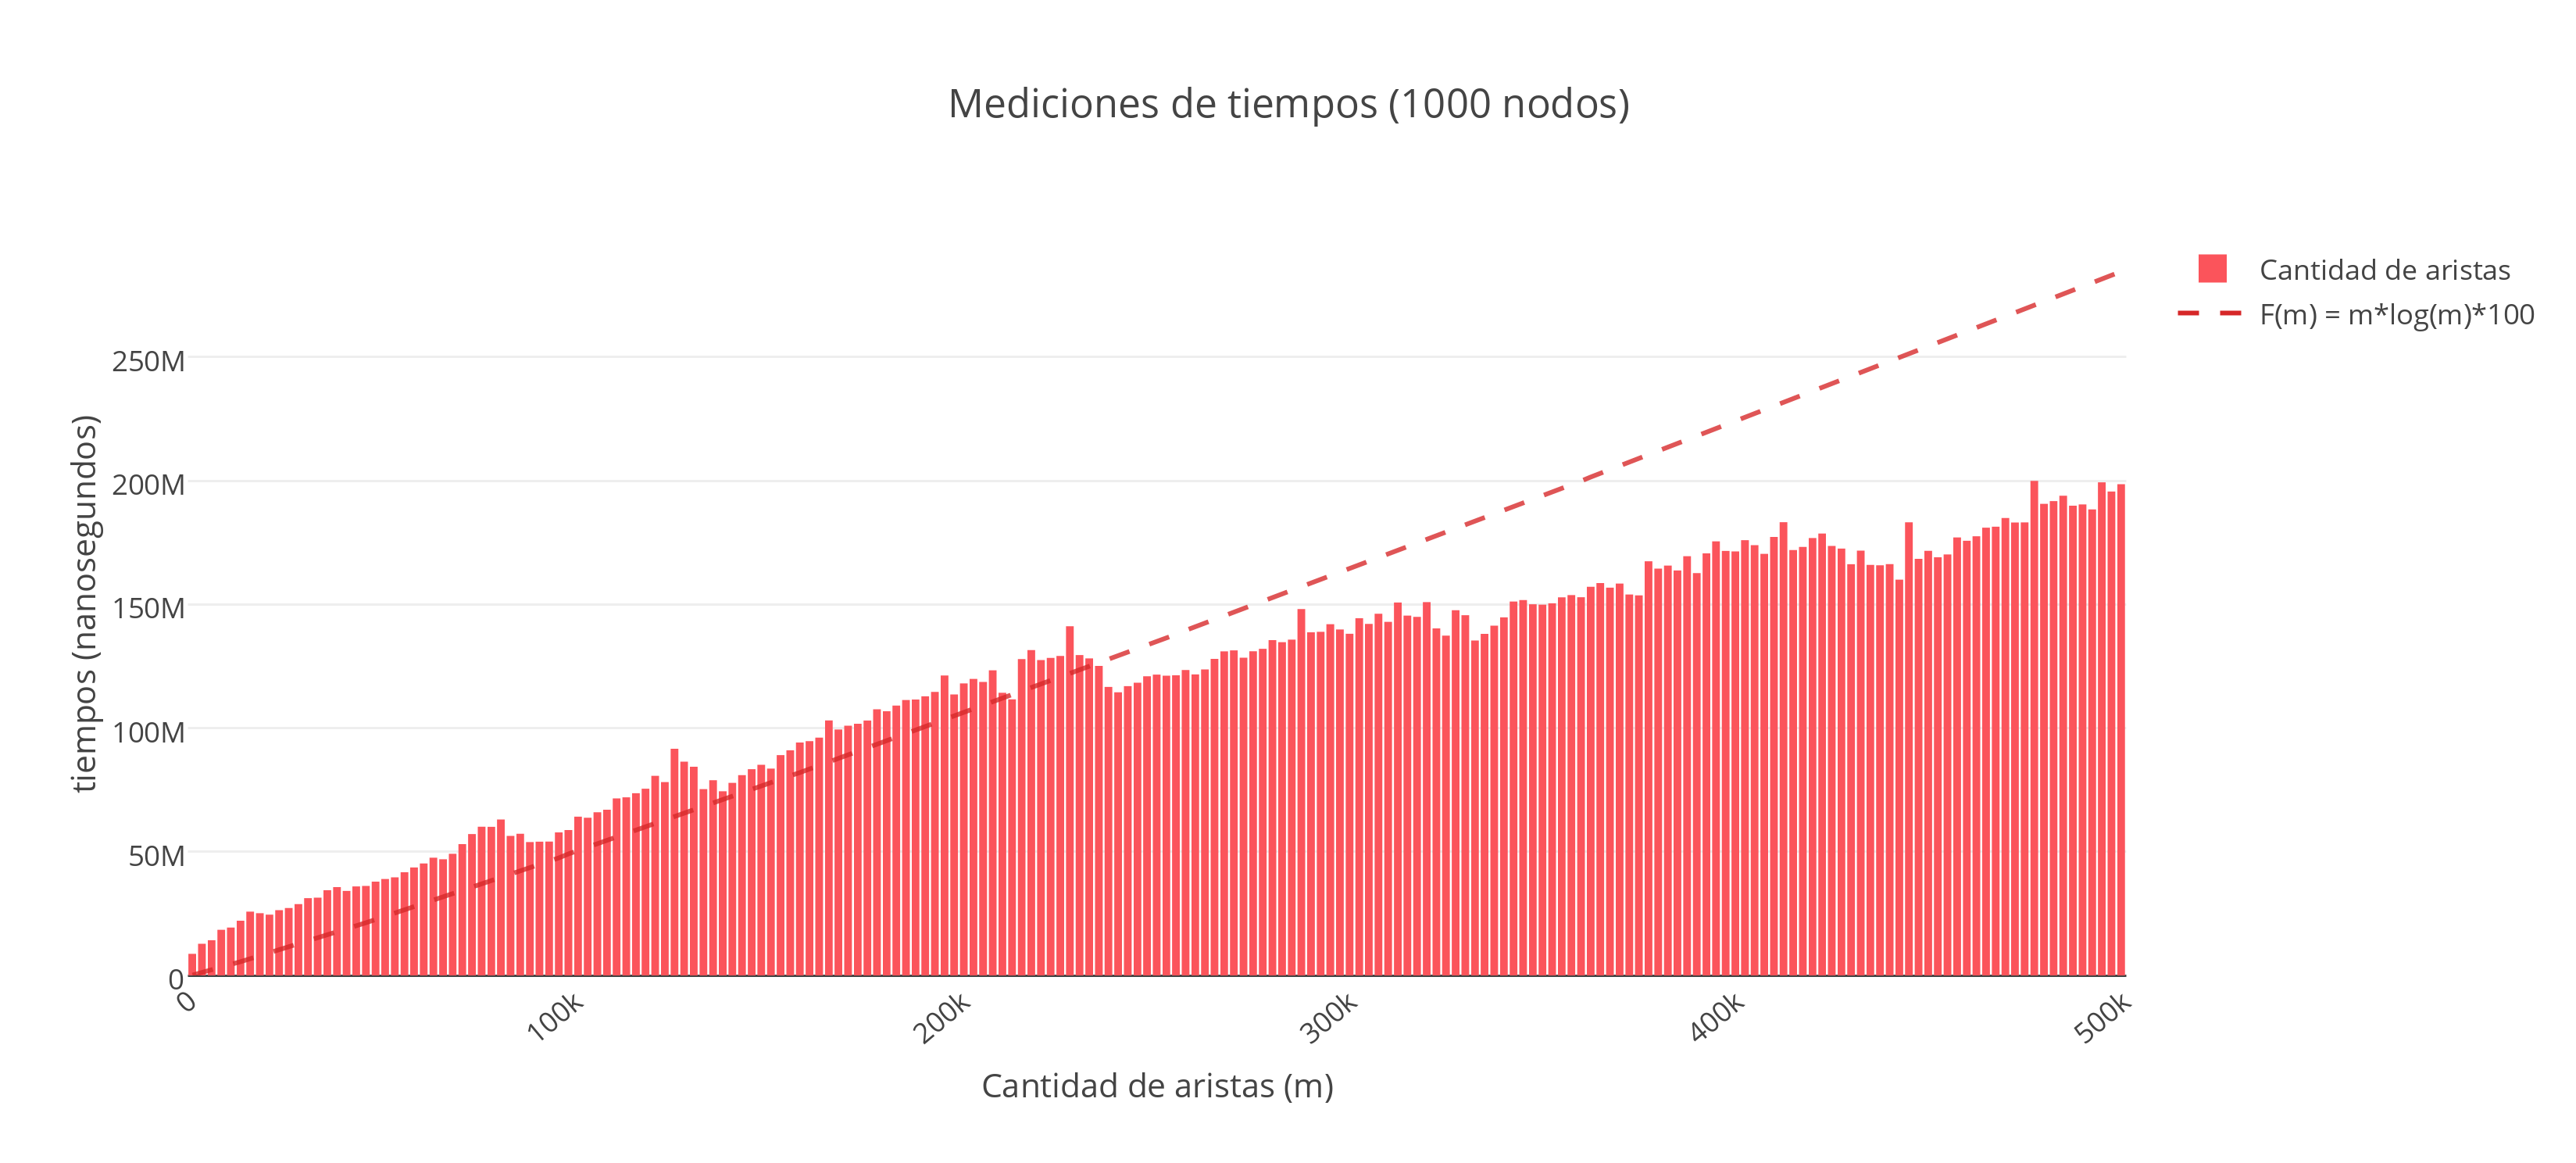
\includegraphics[scale=0.6]{imagenes/ej3/tiempos1000B.png}
% 	\caption{Medición de tiempo promedio con $n$ fijo en 1000}
% 	%\label{tiemposprom}
%  \end{figure}